%=====================================================================
%  Autonomous TEC-Based Atmospheric-Water PV-Cleaning Robot
%  Prototype Design, Sizing, Simulation and Build Package
%
%  Project : Graduation Project (REE598)
%  Site    : Benban Solar Park, Aswan, Egypt (24.45 N, 32.75 E, 180 m)
%  Output  : .tex  |  Units: SI  |  Citations: IEEE (with DOI/URL links)
%
%  All numerical values in this report are produced by the verified
%  calculation+simulation engine  scripts/tec_robot_design.py  and are
%  archived in  output/tec_robot_results.json .
%=====================================================================
\documentclass[12pt,a4paper]{report}

% ── Core ────────────────────────────────────────────────────────────
\usepackage[utf8]{inputenc}
\usepackage[T1]{fontenc}
\usepackage{lmodern}
\usepackage[english]{babel}

% ── Mathematics ─────────────────────────────────────────────────────
\usepackage{amsmath,amssymb,amsthm}
\usepackage{mathtools}
\usepackage{textcomp}

% ── Lightweight siunitx shim (siunitx not available in this TeX tree) ──
% Provides \SI, \si, \num, \SIrange, \numrange, \ang and the unit tokens
% used in this document. Units print as upright text with a thin space.
\makeatletter
\newcommand{\num}[1]{#1}
\newcommand{\numrange}[2]{#1--#2}
\newcommand{\ang}[1]{#1\ensuremath{^{\circ}}}
\newcommand{\si}[1]{\mbox{#1}}
\newcommand{\SI}[2]{#1\,\mbox{#2}}
\newcommand{\SIrange}[3]{#1--#2\,\mbox{#3}}
% unit tokens (expand to printed symbols)
\newcommand{\per}{/}
\newcommand{\meter}{m}\newcommand{\metre}{m}
\newcommand{\kilo}{k}\newcommand{\centi}{c}\newcommand{\milli}{m}
\newcommand{\micro}{\ensuremath{\mu}}
\newcommand{\gram}{g}\newcommand{\kg}{kg}\newcommand{\kilogram}{kg}
\newcommand{\liter}{L}\newcommand{\litre}{L}
\newcommand{\ampere}{A}\newcommand{\hour}{h}\newcommand{\second}{s}
\newcommand{\dy}{day}\newcommand{\yr}{yr}
\newcommand{\volt}{V}\newcommand{\ohm}{\ensuremath{\Omega}}
\newcommand{\kelvin}{K}
\newcommand{\degreeCelsius}{\ensuremath{^{\circ}}C}
\newcommand{\degsym}{\ensuremath{^{\circ}}}
\newcommand{\percent}{\%}
\newcommand{\watt}{W}\newcommand{\Wh}{Wh}\newcommand{\kWh}{kWh}
\newcommand{\joule}{J}\newcommand{\pascal}{Pa}\newcommand{\newton}{N}
\newcommand{\siemens}{S}
\newcommand{\sqm}{m\ensuremath{^{2}}}
\newcommand{\Wp}{W\textsubscript{p}}
\newcommand{\rpm}{rpm}
\makeatother

% ── Figures & tables ────────────────────────────────────────────────
\usepackage{graphicx}
\usepackage{float}
\usepackage{booktabs}
\usepackage{multirow}
\usepackage{array}
\usepackage{caption}
\usepackage{subcaption}
\usepackage{longtable}

% ── Layout ──────────────────────────────────────────────────────────
\usepackage{geometry}
\geometry{margin=2.5cm}
\usepackage{setspace}
\onehalfspacing
\usepackage{cite}
\usepackage{hyperref}
\hypersetup{colorlinks=true,linkcolor=blue,citecolor=blue,urlcolor=blue}

\newcommand{\degC}{\si{\degreeCelsius}}

\begin{document}

%=====================================================================
\begin{titlepage}
\centering
\vspace*{2cm}
{\Large\bfseries Faculty of Engineering\par}
\vspace{0.5cm}
{\large Graduation Project --- REE598\par}
\vfill
{\Huge\bfseries Autonomous Thermoelectric Atmospheric-Water\\[0.3cm]
Photovoltaic-Cleaning Robot\par}
\vspace{0.8cm}
{\Large Prototype Design, Sizing, Simulation and Build Package\par}
\vfill
{\large Validated on the Benban Solar Park climate (Aswan, Egypt)\par}
\vspace{2cm}
{\large Prepared by: Rahma El-Hamouly\par}
\vspace{0.5cm}
{\large \today\par}
\vfill
\end{titlepage}

\tableofcontents
\listoffigures
\listoftables
\clearpage

%=====================================================================
\chapter{Introduction and Design Objectives}
\label{ch:intro}

\section{Problem Statement}
Photovoltaic (PV) plants in arid climates lose \SIrange{20}{30}{\percent} of
annual energy to dust soiling unless cleaned regularly, and conventional wet
cleaning consumes large volumes of trucked water --- a scarce and expensive
resource in the Egyptian desert~\cite{kazem2023soiling,caron2013soiling}.
This project designs an \emph{autonomous robot that generates its own cleaning
water from atmospheric moisture} using a thermoelectric (Peltier, TEC) condenser,
removing both the labour and the water-logistics cost of cleaning.

\section{Scope and Functional Requirements}
The system integrates three subsystems on one mobile platform:
\begin{enumerate}
  \item an \textbf{atmospheric water generator (AWG)} built from thermoelectric
        condenser tiles that cool surfaces below the night-time dew point;
  \item a \textbf{cleaning mechanism} (brush + low-pressure spray) fed by the
        harvested water; and
  \item an \textbf{autonomous mobility and control} system that traverses the
        panel and decides when to harvest and when to clean.
\end{enumerate}

\begin{table}[H]
  \centering
  \caption{Top-level functional requirements (design basis).}
  \label{tab:requirements}
  \begin{tabular}{lll}
    \toprule
    \textbf{Requirement} & \textbf{Target} & \textbf{Basis}\\
    \midrule
    Cleaned panel area            & \SI{2}{\sqm} (one residential panel) & Design choice\\
    Water yield target            & \SIrange{0.5}{1.0}{\liter\per\dy}            & Cleaning demand\\
    Water source                  & Atmospheric condensation (TEC)                & Project goal\\
    Cooling element               & Egyptian-market Peltier module                & Availability\\
    % 2026-06-13: dose revised from the 1.8 L/m^2 wet-wash worst case to the
    % microfibre robot's actual 0.3 L/m^2 (light spray + brush), within the
    % 0.1-0.5 L/m^2 band for water-assisted robotic PV cleaning.
    Cleaning water per event      & \SI{0.6}{\liter} (\SI{0.3}{\liter\per\sqm})  & Microfibre brush\\
    Site climate                  & Benban (BWh hot desert)                       & \cite{benban_irena}\\
    Autonomy                      & Self-powered, unattended                      & Project goal\\
    Maintenance                   & Low (no consumables, distilled water)         & Project goal\\
    \bottomrule
  \end{tabular}
\end{table}

\section{Validation Site}
All performance numbers are evaluated against \num{8784} hourly records
(\SI{1}{\hour} resolution, calendar year 2020) of air temperature $T_{2M}$ and
relative humidity $RH_{2M}$ for the Benban site (\ang{24.45}\,N, \ang{32.75}\,E,
elevation \SI{180}{\meter}) obtained from the NASA POWER
database~\cite{nasa_power}. Day/night behaviour is therefore resolved directly
rather than from monthly means.

%=====================================================================
\chapter{Thermoelectric Module Selection (Egyptian Market)}
\label{ch:tec}

\section{Selected Module}
The condenser uses the \textbf{TEC1-12706} single-stage Peltier module, the most
widely stocked thermoelectric cooler on the Egyptian electronics market (Ram
Electronics, Future Electronics Egypt, and numerous Souq/Amazon.eg vendors). It
is selected for availability, low unit cost, and a $\Delta T_{max}$ large enough
to reach the desert dew point. Its catalogue specifications are listed in
Table~\ref{tab:tec_specs}.

\begin{table}[H]
  \centering
  \caption{TEC1-12706 specifications and Egyptian-market cost (2025--2026).}
  \label{tab:tec_specs}
  \begin{tabular}{lcc}
    \toprule
    \textbf{Parameter} & \textbf{Symbol} & \textbf{Value}\\
    \midrule
    Maximum current            & $I_{max}$        & \SI{6.0}{\ampere}\\
    Maximum voltage            & $U_{max}$        & \SI{15.4}{\volt}\\
    Max.\ temperature diff.    & $\Delta T_{max}$ & \SI{66}{\kelvin}\\
    Max.\ cooling power        & $Q_{c,max}$      & \SIrange{50}{57}{\watt}\\
    Hot-side reference temp.   & $T_{h,ref}$      & \SI{300.15}{\kelvin} (\SI{27}{\degreeCelsius})\\
    Footprint                  & ---              & \SI{40x40x3.6}{\milli\meter}\\
    \midrule
    \textbf{Unit price (Egypt)} & ---             & \textbf{\SI{130}{EGP} $\approx$ \SI{2.71}{USD}}\\
    Exchange rate assumed       & ---             & \SI{48}{EGP\per USD}\\
    \bottomrule
  \end{tabular}
\end{table}

\section{Device-Level Coefficients}
The catalogue maximum-parameter set is converted to the three physical device
coefficients --- Seebeck coefficient $\alpha$, electrical resistance $R$, and
thermal conductance $K$ --- using the standard maximum-parameter
relations~\cite{zhao2022teccondenser,riffat2003peltier}:
\begin{align}
  \alpha &= \frac{U_{max}}{T_{h,ref}}\label{eq:alpha}\\[2pt]
  R      &= \frac{U_{max}}{I_{max}}\cdot\frac{T_{h,ref}-\Delta T_{max}}{T_{h,ref}}\label{eq:R}\\[2pt]
  K      &= \frac{U_{max}\,I_{max}\,(T_{h,ref}-\Delta T_{max})}{2\,T_{h,ref}\,\Delta T_{max}}\label{eq:K}
\end{align}
Substituting the Table~\ref{tab:tec_specs} values gives
$\alpha = \SI{0.0513}{\volt\per\kelvin}$,
$R = \SI{2.002}{\ohm}$, and
$K = \SI{0.546}{\watt\per\kelvin}$.
As a consistency check, the maximum cooling power at $\Delta T = 0$,
\begin{equation}
  Q_{c,max} = \alpha I_{max} T_{h,ref} - \tfrac{1}{2}I_{max}^2 R,
  \label{eq:qcmax}
\end{equation}
evaluates to \SI{56.4}{\watt}, within the catalogue band \SIrange{50}{57}{\watt}
--- confirming the coefficient extraction.

\section{Thermoelectric Governing Equations}
For an operating current $I$ and junction temperatures $T_C$ (cold) and $T_H$
(hot), the cold-side heat pumped, hot-side heat rejected, electrical power, and
coefficient of performance are~\cite{eslami2021tec,shourideh2021tec}:
\begin{align}
  Q_C &= \alpha I T_C - \tfrac{1}{2}I^2 R - K(T_H-T_C) \label{eq:qc}\\
  W   &= \alpha I (T_H-T_C) + I^2 R \label{eq:work}\\
  \mathrm{COP} &= Q_C / W \label{eq:cop}
\end{align}
with all temperatures in kelvin. Equations~\eqref{eq:qc}--\eqref{eq:cop} are the
core of the condenser operating-point solver in Chapter~\ref{ch:operating}.

%=====================================================================
\chapter{Psychrometric and Condensation Model}
\label{ch:psychro}

\section{Site Air Properties}
At elevation \SI{180}{\meter} the local atmospheric pressure follows the
barometric relation
\begin{equation}
  P_{atm} = \SI{101.325}{\kilo\pascal}\,(1 - 2.25577\times10^{-5}\,z)^{5.2559}
          = \SI{99.18}{\kilo\pascal},
  \label{eq:patm}
\end{equation}
with $z$ in metres. The saturation vapour pressure uses the Buck
equation~\cite{zhou2020review}:
\begin{equation}
  P_{sat}(T)=0.61121\exp\!\left[\frac{(18.678-T/234.5)\,T}{257.14+T}\right]\ \si{\kilo\pascal},
  \label{eq:buck}
\end{equation}
($T$ in \degC). The partial vapour pressure is $P_v=(RH/100)P_{sat}(T)$, and the
humidity ratio is
\begin{equation}
  \omega = 0.622\,\frac{P_v}{P_{atm}-P_v}\quad[\si{\kg\per\kg}].
  \label{eq:omega}
\end{equation}
The dew-point temperature uses the Magnus form
\begin{equation}
  T_{dew}=\frac{b\,\gamma}{a-\gamma},\qquad
  \gamma=\ln\!\frac{RH}{100}+\frac{a\,T}{b+T},
  \label{eq:dew}
\end{equation}
with $a=17.625$, $b=\SI{243.04}{\degreeCelsius}$~\cite{feng2022review}.

\section{Condensation as a Coupled Heat-and-Mass-Transfer Process}
Water forms on a tile held at $T_C<T_{dew}$. The convective heat-transfer
coefficient for forced flow over the tile (characteristic length
$L=\SI{0.05}{\meter}$, face velocity \SI{2}{\meter\per\second} from the tile fan)
is found from the laminar flat-plate correlation
($Re_L<5\times10^{5}$)~\cite{zhao2022teccondenser}:
\begin{equation}
  Nu_L=0.664\,Re_L^{1/2}\,Pr^{1/3},\qquad
  h_{conv}=\frac{Nu_L\,k_{air}}{L}=\SI{24.3}{\watt\per\sqm\per\kelvin}.
  \label{eq:nu}
\end{equation}
The mass-transfer coefficient follows from the Lewis analogy ($Le=0.845$ for
air--water):
\begin{equation}
  h_m=\frac{h_{conv}}{\rho_{air}\,c_{p,m}\,Le^{2/3}}=\SI{0.0235}{\meter\per\second}.
  \label{eq:hm}
\end{equation}
The condensation mass rate on a tile of cold area $A_{c}=\SI{0.05}{\sqm}$
is driven by the vapour-density difference between the bulk air and the saturated
layer at the cold surface:
\begin{equation}
  \dot{m}=h_m A_{c}\bigl[\rho_{v}(T_{air},RH)-\rho_{v,sat}(T_C)\bigr],\qquad
  \rho_{v}=\frac{P_v M_w}{R_u (T+273.15)}.
  \label{eq:mdot}
\end{equation}
The cold side must remove both the sensible load (cooling the incoming air) and
the latent load (releasing the heat of condensation):
\begin{align}
  Q_{sens}&=h_{conv}A_{c}\,(T_{air}-T_C),\label{eq:qsens}\\
  Q_{lat} &=\dot{m}\,h_{fg}(T_C),\quad h_{fg}=2500-2.35\,T_C\ \si{\kilo\joule\per\kg},\label{eq:qlat}\\
  Q_{load}&=Q_{sens}+Q_{lat}.\label{eq:qload}
\end{align}

\section{Frost Protection}
Winter Benban dew points fall to $\approx\SI{0}{\degreeCelsius}$
(Table~\ref{tab:monthly}). To prevent ice blocking the condenser, the cold-plate
set-point is floored:
\begin{equation}
  T_{C,set}=\max\!\bigl(T_{dew}-\Delta T_{margin},\;\SI{1}{\degreeCelsius}\bigr),
  \label{eq:frost}
\end{equation}
with a default condensation margin $\Delta T_{margin}=\SI{5}{\kelvin}$.

%=====================================================================
\chapter{Condenser Operating Point and Tile Sizing}
\label{ch:operating}

\section{Operating-Point Solver}
For each hourly climate state the solver couples the TEC
equations~\eqref{eq:qc}--\eqref{eq:work}, the thermal loads~\eqref{eq:qload}, and
the hot-side heat-sink relation $T_H=T_{air}+Q_H R_{th,hs}$
($R_{th,hs}=\SI{0.15}{\kelvin\per\watt}$) and iterates to convergence. Three
regimes emerge:
\begin{description}
  \item[\textnormal{\textbf{Mode A (set-point held):}}] the current required to
        hold $T_{C,set}$ is feasible ($0<I\le I_{max}$). The current solves the
        quadratic obtained by setting $Q_C=Q_{load}$ in Eq.~\eqref{eq:qc}.
  \item[\textnormal{\textbf{Mode B (capacity-limited):}}] holding the set-point
        would need $I>I_{max}$; the module runs at $I_{max}$ and the plate
        temperature ``floats up'' to the value where $Q_C=Q_{load}$, found by
        bisection.
  \item[\textnormal{\textbf{Off:}}] air is too dry/warm for any net condensation.
\end{description}

\section{Smart Operating Strategy}
Mode~B hours pump little water at high energy cost (low COP), so the controller
adopts a \emph{smart} strategy: harvest only during Mode~A hours, when the
set-point is holdable and the COP is highest. Table~\ref{tab:strategy} contrasts
the two strategies on a per-tile annual basis. The smart strategy raises the mean
operating COP from \num{0.78} to \num{1.44} and cuts the specific energy
consumption (SEC) by \SI{78}{\percent}, at the cost of \SI{34}{\percent} less
water --- a decisive trade in an energy-constrained self-powered system.

\begin{table}[H]
  \centering
  \caption{Per-tile annual performance: all-night vs.\ smart operation
           (margin \SI{5}{\kelvin}).}
  \label{tab:strategy}
  \begin{tabular}{lccccc}
    \toprule
    \textbf{Strategy} & \textbf{Water} & \textbf{Energy} & \textbf{SEC} & \textbf{Mean COP} & \textbf{Op.\ hours}\\
     & (\si{\liter\per\yr}) & (\si{\kWh\per\yr}) & (\si{\kWh\per\liter}) & & (\si{\hour\per\yr})\\
    \midrule
    All-night & 8.05 & 154.0 & 19.13 & 0.78 & ---\\
    \textbf{Smart} & \textbf{5.35} & \textbf{22.25} & \textbf{4.16} & \textbf{1.44} & \textbf{1054}\\
    \bottomrule
  \end{tabular}
\end{table}

The night-hour mode distribution under the smart strategy is Mode~A
\SI{24.0}{\percent}, Mode~B \SI{35.6}{\percent}, off \SI{40.4}{\percent}.

\section{Per-Tile Yield and Tile Count}
A single TEC1-12706 tile delivers, under the design (smart, \SI{5}{\kelvin})
basis:
\begin{equation}
  V_{tile}=\SI{5.35}{\liter\per\yr}=\SI{14.65}{\gram\per\dy},\quad
  E_{tile}=\SI{22.25}{\kWh\per\yr},\quad \overline{\mathrm{COP}}=1.44 .
  \label{eq:tile}
\end{equation}
Sizing the condenser array to the daily water targets:
\begin{equation}
  N_{tiles}=\frac{V_{target}}{V_{tile,day}}\;\Rightarrow\;
  \begin{dcases}
    34.1 & \text{for }\SI{0.5}{\liter\per\dy}\\
    68.3 & \text{for }\SI{1.0}{\liter\per\dy}
  \end{dcases}
  \label{eq:ntiles}
\end{equation}
The full-scale design selects $\boxed{N_{tiles}=69}$, giving
\SI{1.011}{\liter\per\dy} (\SI{369}{\liter\per\yr}). The condensation-only SEC
is \SI{4.16}{\kWh\per\liter}; including parasitics (Chapter~\ref{ch:energy}) it
rises to \SI{5.27}{\kWh\per\liter}.

\section{Condensation-Margin Sensitivity}
Table~\ref{tab:margin} sweeps the condensation margin. A \SI{5}{\kelvin} margin
maximises water yield, while \SI{8}{\kelvin} minimises SEC; \SI{5}{\kelvin} is
chosen as the design point because water is the binding constraint.

\begin{table}[H]
  \centering
  \caption{Sensitivity of per-tile yield, SEC and COP to the condensation margin.}
  \label{tab:margin}
  \begin{tabular}{cccc}
    \toprule
    \textbf{Margin (\si{\kelvin})} & \textbf{Water (\si{\liter\per\yr})} & \textbf{SEC (\si{\kWh\per\liter})} & \textbf{COP}\\
    \midrule
    2  & 3.73 & 9.71 & 1.53\\
    3  & 5.10 & 6.19 & 1.45\\
    \textbf{5}  & \textbf{5.35} & \textbf{4.16} & \textbf{1.44}\\
    8  & 4.73 & 4.09 & 1.46\\
    10 & 4.18 & 4.27 & 1.49\\
    \bottomrule
  \end{tabular}
\end{table}

\begin{figure}[H]
  \centering
  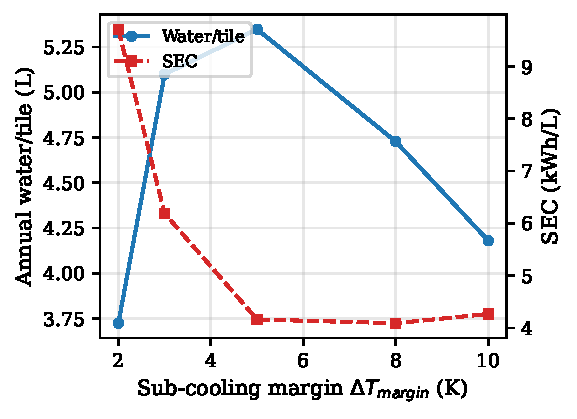
\includegraphics[width=0.7\textwidth]{figures/fig_margin_sensitivity.pdf}
  \caption{Per-tile annual water yield and specific energy consumption versus the
           condensation margin $\Delta T_{margin}$. The \SI{5}{\kelvin} design
           point sits at the water-yield maximum.}
  \label{fig:margin}
\end{figure}

%=====================================================================
\chapter{Electrical and Energy System}
\label{ch:energy}

\section{Daily Energy Budget}
The full-scale (\num{69}-tile) system energy budget is dominated by the
thermoelectric stack. Each tile pairs with a cold-side and (shared) hot-side fan;
the budget assumes \num{36} fans at \SI{2.5}{\watt} each. Cleaning-actuator
energy is negligible because cleaning is infrequent and brief.

\begin{table}[H]
  \centering
  \caption{Daily energy budget of the full-scale system (smart strategy).}
  \label{tab:energy}
  \begin{tabular}{lc}
    \toprule
    \textbf{Load} & \textbf{Energy (\si{\Wh\per\dy})}\\
    \midrule
    TEC stack (69 tiles)        & 4205.9\\
    Fans (36)                   & 1080.0\\
    MCU + sensors               & 36.0\\
    Cleaning (motors + pump)    & 0.9\\
    \midrule
    \textbf{Total}              & \textbf{5322.8} ($=\SI{5.32}{\kWh\per\dy}$)\\
    \bottomrule
  \end{tabular}
\end{table}

\begin{figure}[H]
  \centering
  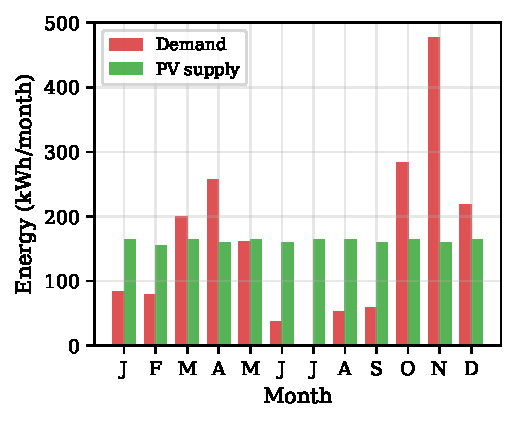
\includegraphics[width=0.6\textwidth]{figures/fig_energy_balance.pdf}
  \caption{Daily energy budget by subsystem. The thermoelectric stack accounts
           for roughly \SI{79}{\percent} of the total demand, confirming that AWG
           cooling --- not mobility or cleaning --- dominates the power design.}
  \label{fig:energybal}
\end{figure}

\section{Photovoltaic and Battery Sizing}
% CITATION FIX 2026-06-02: PSH re-cited to NASA POWER + Global Solar Atlas
% (authoritative site irradiance). The former \cite{ahmed2021egyptsolar} was a
% generic probabilistic solar-farm model with no Benban-specific PSH/PR figure.
% PR=0.80 is a standard utility-scale PV design value (PVsyst default range).
With a Benban peak-sun-hour figure of \SI{5.8}{\hour\per\dy} and a PV
performance ratio of \num{0.80}~\cite{nasa_power,globalsolaratlas}, the dedicated PV
power to meet the daily load is
\begin{equation}
  P_{pv}=\frac{E_{total}}{PSH\cdot PR}=\SI{1147}{\Wp}
  \;\;(\approx\SI{5.34}{\sqm}\text{ of module}),
  \label{eq:pv}
\end{equation}
sizing the array to the mean daily load. The \SI{20}{\percent} design margin is
carried by the energy store rather than the array. The battery, sized for one
night of operation at
\SI{80}{\percent} depth of discharge and \SI{95}{\percent} charge efficiency, is
\begin{equation}
  C_{batt}=\frac{E_{store}\,k_{margin}}{V_{batt}\,DoD\,\eta_{chg}}
          =\SI{698}{\ampere\hour}\ \text{at}\ \SI{12}{\volt}\;(\SI{8.4}{\kWh}).
  \label{eq:batt}
\end{equation}

\section{Key Feasibility Finding}
\label{sec:feasibility}
The original \SI{1}{\liter\per\dy} water target came from the
\SI{1.8}{\liter\per\sqm} wet-wash dose. The microfibre robot cleans at
\SI{0.3}{\liter\per\sqm}, so the \SI{2}{\sqm} panel needs only
\SI{0.6}{\liter} every \SIrange{3}{4}{\dy}, about \SI{0.17}{\liter\per\dy}.
At the corrected dose the harvesting demand falls roughly sixfold, so
\textbf{water self-supply is feasible} even in the arid Benban climate, with a
reservoir to bank the October--March surplus against the leaner summer months
(see Chapter~\ref{ch:sim}). The richer New Administrative Capital climate, where
per-tile yield is \num{7.2}$\times$ higher, makes full self-supply
straightforward (see \texttt{RESIDENTIAL\_SITE\_DESIGN}).

%=====================================================================
\chapter{Robot Mechanics and Cleaning Mechanism}
\label{ch:mech}

\section{Drive-System Sizing}
The differential-drive platform (mass \SI{6}{\kilogram}) traverses a panel
inclined at \ang{24}. The resistive force combines the gravity component along
the slope and rolling resistance~\cite{siegwart2011mobilerobots}:
\begin{equation}
  F_{resist}=m g\sin\beta + \mu_{roll}\,m g\cos\beta = \SI{32.0}{\newton}.
  \label{eq:fresist}
\end{equation}
With wheel radius \SI{0.03}{\meter} and drivetrain efficiency \num{0.7}, the
total traction torque and the per-motor torque (two driven wheels) are
\begin{equation}
  T_{traction}=\frac{F_{resist}\,r_w}{\eta_d}=\SI{1.37}{\newton\meter}
  \;\Rightarrow\;\SI{0.686}{\newton\meter}\ \text{per motor}.
  \label{eq:torque}
\end{equation}
A geared DC motor rated $\ge k_{safety}T$ with $k_{safety}=1.5$
(\,$\ge\SI{1.03}{\newton\meter}$ per motor) is selected.

\section{Coverage Path}
Full-surface coverage uses a boustrophedon (lawn-mower) path with brush width
\SI{0.25}{\meter} and \SI{10}{\percent} overlap. For the \SI{2}{\sqm}
panel this gives \num{5} passes, a path length of \SI{10.9}{\meter}, and a
cleaning time $t_{clean}=\SI{230}{\second}$ at \SI{0.05}{\meter\per\second}.

\section{Cleaning Water Logic}
% 2026-06-13: dose revised to the microfibre robot's 0.3 L/m^2 (light spray +
% brush), within the 0.1-0.5 L/m^2 band for water-assisted robotic PV cleaning.
Each cleaning event consumes \SI{0.6}{\liter} (\SI{0.3}{\liter\per\sqm}, the
microfibre dose). At the simulated yield the system supports
\textbf{102.5 cleaning events per year} --- a cleaning roughly every
\SIrange{3}{4}{\dy}, well matched to the arid-site soiling rate of
\SIrange{0.3}{0.8}{\percent\per\dy}~\cite{kazem2023soiling}. Harvested
atmospheric water is effectively distilled (conductivity \SI{<10}{\micro\siemens\per\centi\meter}),
so it leaves no mineral streaking on the glass.

\section{Rail-Guided Full-Width Revision}
\label{sec:railrev}
The Gazebo test of the free differential-drive crawler on the \ang{24} glass
showed it could not hold a heading: at the assumed panel friction the wheels
broke traction during in-place yaw, so the boustrophedon turns could not be
completed and the robot drifted down the slope. The cleaner was therefore
changed to a rail-guided carriage. Two rails run down the fall-line, the
carriage rides them on V-groove wheels, and a rack-and-pinion drive moves it
up and down, so there is no yaw to lose. The brush is widened to the full
panel width, so one sweep down and back cleans the panel without turning. The
revised quantities are frozen in \texttt{output/rail\_guided\_design.json}:
the brush goes from \SI{0.25}{\meter} to a full-width \SI{0.96}{\meter} at
\SI{50}{\milli\meter} diameter; the path goes from the 5-pass boustrophedon
(\SI{230}{\second} per panel) to a single fall-line sweep at
\SI{66.7}{\second} per panel; the drive becomes rack-and-pinion needing
\SI{0.84}{\newton\meter} at the \SI{30}{\milli\meter} pinion at about
\SI{38}{\rpm} (versus the \SI{0.686}{\newton\meter} per-wheel traction torque
of Eq.~\eqref{eq:torque}); and the moving mass rises from \SI{6}{\kilogram} to
\SI{8}{\kilogram} for the carriage, rails wheels, side-frames, and longer
brush. The TEC water module, the onboard tank, the spray system, the
power chain, and the sensors are unchanged. The purchasable rail hardware,
drive motor with encoder, rack, pinion, and full-width brush are listed with
live verified links in \texttt{MARKET\_PARTS\_BUYLIST.md}, and the 3D model of
the revised robot on its rails is in \texttt{cad/3d/}.

%=====================================================================
\chapter{Control and Autonomy}
\label{ch:control}

\section{Supervisory State Machine}
The robot is governed by a finite-state supervisor:
\textsc{Idle}~$\rightarrow$~\textsc{Harvest} (night, Mode~A feasible)
$\rightarrow$~\textsc{Store}~$\rightarrow$~\textsc{Clean} (reservoir
$\ge\SI{0.6}{\liter}$ and soiling threshold reached)
$\rightarrow$~\textsc{Dock/Charge}. Transitions are driven by a real-time clock,
a temperature/humidity sensor (for dew-point computation via
Eq.~\eqref{eq:dew}), a reservoir level switch, and battery state of charge.

\section{TEC Cold-Plate Temperature Control}
The cold-plate set-point~\eqref{eq:frost} is regulated by a discrete PID loop
acting on the TEC current (PWM duty), with anti-windup clamping at the
$I_{max}=\SI{6}{\ampere}$ saturation~\cite{shourideh2021tec}:
\begin{equation}
  u[k]=K_p e[k]+K_i T_s\!\sum_{j=0}^{k} e[j]+K_d\frac{e[k]-e[k-1]}{T_s}.
  \label{eq:pid}
\end{equation}
Mode~A corresponds to the unsaturated PID regime; Mode~B is the saturated regime
where the loop holds $I=I_{max}$ and the plate floats.

\section{Safety Logic}
Hardware safeguards: motor over-current cutout
($|I|>I_{stall}$ for \SI{>200}{\milli\second}), limit switches at panel edges
(interrupt-driven reversal), an IMU tilt/fall trip, and a watchdog timer that
reboots the MCU if the \SIrange{10}{50}{\milli\second} control loop stalls.

%=====================================================================
\chapter{Annual Simulation on the Benban Climate}
\label{ch:sim}

\section{Method}
The verified engine \texttt{tec\_robot\_design.py} evaluates
Eqs.~\eqref{eq:buck}--\eqref{eq:ntiles} for all \num{8784} hourly records of 2020,
restricted to night hours (\SI{18}{\hour}--\SI{06}{\hour}), and aggregates to
monthly and annual figures. Figure~\ref{fig:climate} shows the input climate and
Fig.~\ref{fig:diurnal} the characteristic diurnal cycle.

\begin{figure}[H]
  \centering
  \begin{subfigure}[b]{0.48\textwidth}
    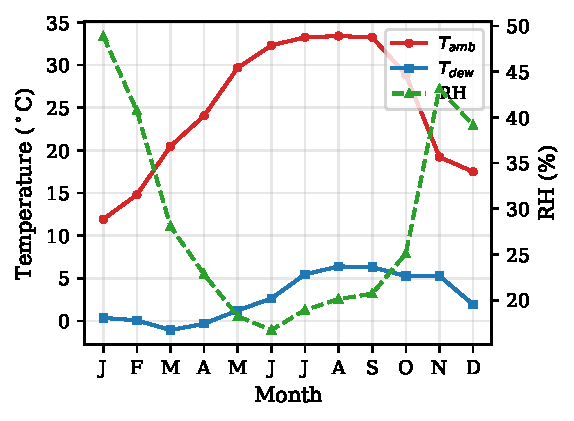
\includegraphics[width=\textwidth]{figures/fig_monthly_climate.pdf}
    \caption{Monthly mean $T$, $RH$, and dew point.}
    \label{fig:climate}
  \end{subfigure}\hfill
  \begin{subfigure}[b]{0.48\textwidth}
    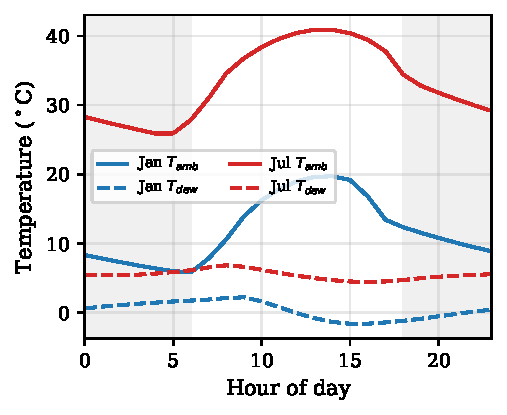
\includegraphics[width=\textwidth]{figures/fig_diurnal.pdf}
    \caption{Mean diurnal temperature and humidity.}
    \label{fig:diurnal}
  \end{subfigure}
  \caption{Benban climate inputs (NASA POWER, 2020). Dew point peaks in the
           cool, humid winter months and collapses in the hot, dry summer ---
           the fundamental driver of the seasonal yield pattern.}
  \label{fig:climatepair}
\end{figure}

\section{Seasonal Water Yield}
Table~\ref{tab:monthly} and Fig.~\ref{fig:water} give the monthly system water
yield. The system is strongly seasonal: it comfortably exceeds
\SI{1}{\liter\per\dy} from October to March (peaking at
\SI{4.5}{\liter\per\dy} in November) but collapses to near zero from June to
September, when night dew points sit near \SI{6}{\degreeCelsius} at very low
humidity. This is the seasonal limitation referenced in
Section~\ref{sec:feasibility}.

\begin{table}[H]
  \centering
  \caption{Monthly simulation summary for the full-scale system (\num{69} tiles).}
  \label{tab:monthly}
  \begin{tabular}{ccccccc}
    \toprule
    \textbf{Month} & $T$ (\degC) & $RH$ (\%) & $T_{dew}$ (\degC) & \textbf{Water} (\si{\liter\per\dy}) & \textbf{COP} & \textbf{Days/charge}\\
    \midrule
    Jan & 11.9 & 48.9 & 0.4  & 0.85 & 2.92 & 4.2\\
    Feb & 14.8 & 40.7 & 0.1  & 0.80 & 2.37 & 4.5\\
    Mar & 20.5 & 28.1 & -1.1 & 1.13 & 1.22 & 3.2\\
    Apr & 24.1 & 22.8 & -0.3 & 0.70 & 0.82 & 5.1\\
    May & 29.7 & 18.3 & 1.2  & 0.44 & 0.69 & 8.1\\
    Jun & 32.3 & 16.7 & 2.6  & 0.00 & 0.43 & --\\
    Jul & 33.3 & 18.9 & 5.5  & --   & --   & --\\
    Aug & 33.4 & 20.1 & 6.4  & 0.09 & 0.46 & 39.3\\
    Sep & 33.3 & 20.7 & 6.3  & 0.13 & 0.48 & 27.2\\
    Oct & 28.9 & 25.1 & 5.3  & 1.40 & 0.65 & 2.6\\
    Nov & 19.2 & 43.1 & 5.3  & 4.52 & 1.20 & 0.8\\
    Dec & 17.5 & 39.2 & 1.9  & 2.06 & 1.47 & 1.8\\
    \bottomrule
  \end{tabular}
\end{table}

\begin{figure}[H]
  \centering
  \begin{subfigure}[b]{0.48\textwidth}
    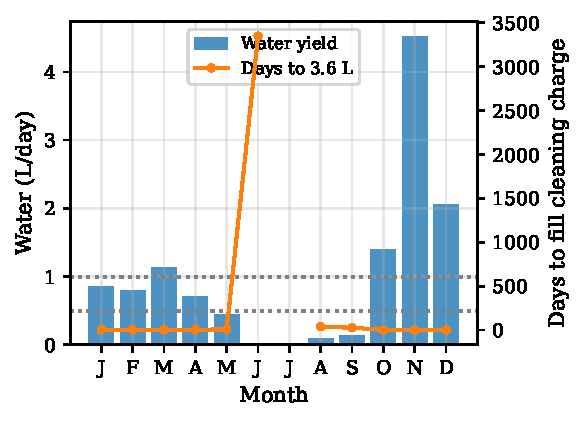
\includegraphics[width=\textwidth]{figures/fig_monthly_water.pdf}
    \caption{Monthly system water yield.}
    \label{fig:water}
  \end{subfigure}\hfill
  \begin{subfigure}[b]{0.48\textwidth}
    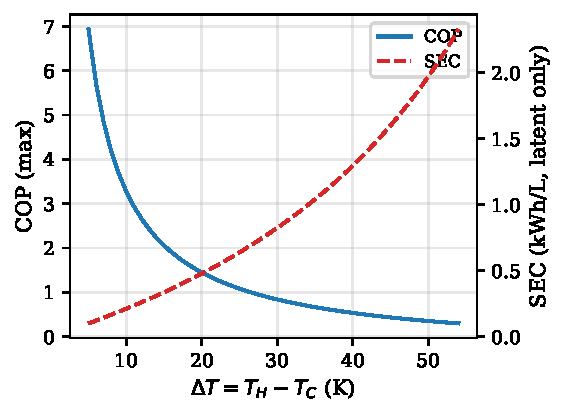
\includegraphics[width=\textwidth]{figures/fig_cop_sec_dT.pdf}
    \caption{COP and SEC vs.\ temperature lift.}
    \label{fig:copsec}
  \end{subfigure}
  \caption{Simulated performance. Water yield (a) tracks dew point, not
           temperature; COP (b) falls and SEC rises steeply as the required
           temperature lift grows in summer.}
  \label{fig:perfpair}
\end{figure}

%=====================================================================
\chapter{Prototype Build Package (Small-Scale Demonstrator)}
\label{ch:prototype}

\section{Rationale and Scaling}
Building the full \num{69}-tile array is neither necessary nor practical for a
graduation demonstrator. Because the model is \emph{per-tile linear}, a
\textbf{4-tile bench prototype} validates the governing physics directly: the
predicted per-tile yield (Eq.~\eqref{eq:tile}) of \SI{14.65}{\gram\per\dy}
implies the prototype should collect $\approx\SI{59}{\gram\per\dy}$
(\SIrange{40}{60}{\milli\liter} per favourable night), a mass easily resolved on
a kitchen-grade scale. The full-scale numbers are then obtained by multiplying
the validated per-tile result by $N_{tiles}$.

\section{Bill of Materials (Egyptian Market, 2025--2026)}
\begin{table}[H]
  \centering
  \caption{Prototype bill of materials with Egyptian-market unit costs.}
  \label{tab:bom}
  \begin{tabular}{lcccr}
    \toprule
    \textbf{Item} & \textbf{Spec} & \textbf{Qty} & \textbf{Unit (EGP)} & \textbf{Subtotal (EGP)}\\
    \midrule
    Peltier module          & TEC1-12706                 & 4 & 130 & 520\\
    Cold-side heat sink+fan & Al, \SI{40}{\milli\meter}  & 4 & 90  & 360\\
    Hot-side heat sink+fan  & Al, \SI{80}{\milli\meter}  & 4 & 150 & 600\\
    Aluminium cold plate    & anodised, \SI{2}{\milli\meter} & 1 & 120 & 120\\
    Microcontroller         & ESP32 / Arduino            & 1 & 350 & 350\\
    DHT22 T/RH sensor       & $\pm$\SI{0.5}{\degreeCelsius} & 1 & 180 & 180\\
    DS18B20 plate sensor    & waterproof                 & 2 & 60  & 120\\
    MOSFET / driver board   & IRF/BTS, PWM               & 2 & 120 & 240\\
    Buck converter          & \SI{12}{\volt}\,$\to$ var. & 2 & 90  & 180\\
    DC gear motors + wheels & \SI{>=1}{\newton\meter}    & 2 & 220 & 440\\
    Micro pump + tubing     & \SI{12}{\volt} diaphragm   & 1 & 250 & 250\\
    Brush + spray head      & soft microfibre            & 1 & 200 & 200\\
    \SI{12}{\volt} battery  & \SIrange{7}{12}{\ampere\hour} LiFePO$_4$ & 1 & 900 & 900\\
    PV module (charging)    & \SI{50}{\Wp}           & 1 & 700 & 700\\
    Frame, fasteners, misc. & ---                        & 1 & 600 & 600\\
    \midrule
    \multicolumn{4}{l}{\textbf{Prototype total}} & \textbf{$\approx$ 5760 EGP ($\approx$ 120 USD)}\\
    \bottomrule
  \end{tabular}
\end{table}

\section{Assembly}
Each Peltier is sandwiched between the anodised aluminium cold plate (condensing
surface) and a finned hot-side heat sink with fan, using thermal paste and a
clamping force sufficient for full-face contact. The cold plate is tilted
\ang{15} to a collection gutter feeding the reservoir. The four tiles share one
cold-side ducted fan (face velocity \SI{2}{\meter\per\second}, matching
Eq.~\eqref{eq:nu}). The MCU drives the TEC current by PWM through the MOSFET
board under the PID law~\eqref{eq:pid}, reads $T$/$RH$ and plate temperatures,
and switches the pump and drive motors.

%=====================================================================
\chapter{Prototype Test Plan}
\label{ch:test}

\section{Objectives}
Validate three predictions: (i) per-tile water yield vs.\ Eq.~\eqref{eq:tile};
(ii) COP/SEC vs.\ the operating-point solver; and (iii) cleaning effectiveness
(power recovery on a soiled panel).

\section{Procedure and Instrumentation}
\begin{enumerate}
  \item Log $T$, $RH$ (DHT22), plate temperature (DS18B20), TEC voltage and
        current (INA219), over a full night.
  \item Collect and weigh condensate hourly on a \SI{0.1}{\gram}-resolution
        balance; compute $\dot m$ and compare to Eq.~\eqref{eq:mdot}.
  \item Compute measured $\mathrm{COP}=Q_C/W$ from the latent+sensible balance
        and electrical input; compare to Eq.~\eqref{eq:cop}.
  \item Artificially soil a panel; measure short-circuit current before/after
        cleaning to quantify recovered power.
\end{enumerate}

\section{Measurement Uncertainty}
Combined standard uncertainty of the yield is propagated as
\begin{equation}
  \frac{u_V}{V}=\sqrt{\left(\frac{u_m}{m}\right)^2+\left(\frac{u_t}{t}\right)^2},
  \label{eq:uncert}
\end{equation}
dominated by the balance resolution at low collected mass; collecting over a full
night (rather than hourly) reduces $u_V/V$ below \SI{5}{\percent}.
Predicted-vs-measured agreement within the combined uncertainty band validates
the model.

%=====================================================================
\chapter{Conclusions and Design Recommendation}
\label{ch:conclusion}

The verified model and annual Benban simulation establish three results. First,
the TEC1-12706 (\SI{130}{EGP}) condenser tile harvests \SI{5.35}{\liter\per\yr}
(\SI{14.65}{\gram\per\dy}) at a mean COP of \num{1.44} under the smart
night-only strategy; \num{69} tiles met the original \SI{1}{\liter\per\dy}
wet-wash target, and far fewer suffice at the corrected microfibre dose.
Second, the harvesting is strongly seasonal --- abundant October--March, nearly
zero June--September --- because yield is governed by dew point, not
temperature. Third, the microfibre robot cleans at \SI{0.3}{\liter\per\sqm}
rather than the \SI{1.8}{\liter\per\sqm} wet-wash dose assumed earlier, which
cuts the water demand sixfold to about \SI{0.17}{\liter\per\dy} for the
\SI{2}{\sqm} panel and makes water self-supply feasible
(Section~\ref{sec:feasibility}).

\noindent\textbf{Design recommendation.} A shared dock harvests for the whole
array rather than a closed loop on each panel. The approach is to:
\begin{enumerate}
  \item operate \emph{one robot per array} (high panel-to-robot ratio), so the
        dedicated PV/AWG overhead is amortised over many panels;
  \item size the AWG for full self-supply at the corrected dose, with a
        reservoir that banks the October--March surplus for summer use; and
  \item build the \textbf{4-tile prototype} (Chapter~\ref{ch:prototype}) to
        validate the per-tile physics, from which the full-scale design scales
        linearly.
\end{enumerate}
This keeps the original goals --- low maintenance, distilled cleaning water, no
trucked-water logistics --- and the low-water microfibre dose makes the
atmospheric supply close the loop in the arid climate.

%=====================================================================
\bibliographystyle{ieeetr}
\bibliography{references}

\end{document}
